%%%%% Design %%%%%
\section{Design} 
%%%%% Structural Design %%%%%
\subsection{Structural Design}
The novel Continuous Six-degree-of-freedom Manipulator introduced in this paper, which corresponds to the scheme design 
shown in Figure \ref{fig:fishboneCR_2023bio}, belongs to the class of bio-inspired continuum robots \cite{fishboneCR}. 
In the design process, a nylon cable drive mechanism is employed as a substitute for the complex musculature of fish, 
enabling it to maintain stability while undergoing deformation movements, thus achieving effective deformation motion 
and controllability. As depicted in Figure \ref{fig:main_components}, the rigid cross-shaped sheets is utilized to mimic 
the spine and ribs, uniformly arranging these sheets on a rubber pure soft sleeve to replace the spinal joints.
\begin{figure}[H] % figure
    \centering
    \captionsetup{labelsep=colon}
    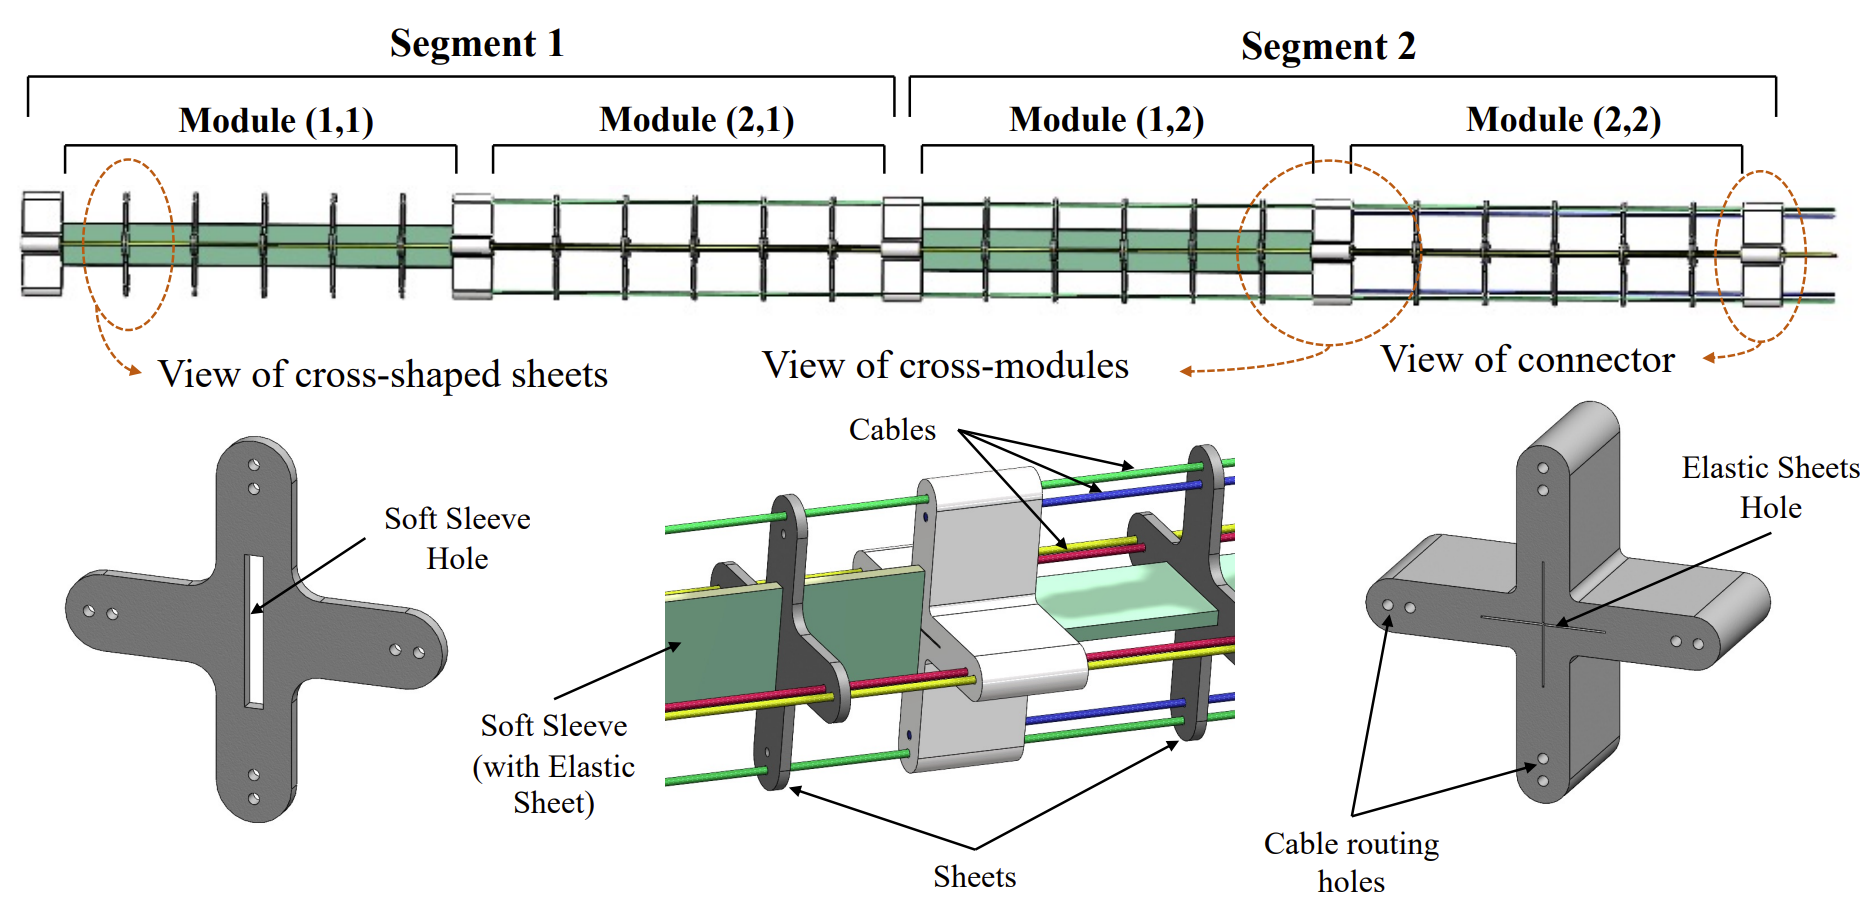
\includegraphics[width=1.0\textwidth]{Image/Design/main_component_of_manipulator.png} 
    \caption[The main components of proposed manipulator and cables arrangement]
    {\centering \textbf{The main components of proposed manipulator and cables arrangement.}}
    \label{fig:main_components}
\end{figure}
%%%%% Parameter Define %%%%%
\subsection{Designation and Parameter Definition of Manipulator}
The manipulator is composed of four identical modules, each of which can be independently controlled to bend within a 
two-dimensional space. Each module consists of an elastic sheet and five uniformly arranged cross-shaped sheets, where 
the rubber pure soft sleeve outside the elastic sheet is interference-fitted with the cross-shaped sheets. The connector 
end of each module features two symmetrically arranged inextensible cables that pass through the cross-shaped sheets and 
are anchored to the connector, driving the end of each manipulator module. By applying tension to one of these cables, 
the elastic sheet can be deflected, thereby achieving a single degree of freedom planar motion at the end of the 
manipulator module. Since the elastic sheets of the modules are transversely mounted, the deflection of two or more 
sheets simultaneously allows for spatial motion at the end of the manipulator, as shown in Figure \ref{fig:main_components}. 
Overall, the proposed manipulator comprises two segments, each maintaining a constant length of 675 mm and a weight of 
88 grams. Each module contains five cross-shaped sheets with a circumferential radius of 20 mm and a thickness of 1.5 mm. 
Both the head and the tail of each segment are connected by connectors, which have the same circumferential radius as 
the cross-shaped sheet and a thickness of 15 mm.

The definition of manipulator parameters is presented in Table \ref{tab:parameter_name}. The subsequent sections 
will adhere to the corresponding naming conventions.
\begin{center}
    \small
    \begin{longtable}{l l l }
    \caption{The Parameters of Manipulators.} \label{tab:parameter_name} \\
    \hline \multicolumn{1}{l}{\textbf{Paramter}} & 
    \multicolumn{1}{l}{\textbf{Definition}} & 
    \multicolumn{1}{l}{\textbf{Value (mm)}} \\ \hline 
    \endfirsthead
    \multicolumn{3}{c}%
    {{\bfseries \tablename\ \thetable{} -- continued from previous page}} \\
    \hline \multicolumn{1}{l}{\textbf{Paramter}} & 
    \multicolumn{1}{l}{\textbf{Definition}} & 
    \multicolumn{1}{l}{\textbf{Value (mm)}} \\ \hline 
    \endhead
    \hline \multicolumn{3}{|r|}{{Continued on next page}} \\ \hline
    \endfoot
    \hline \hline
    \endlastfoot
    % table context
    $Sr_i$       & the length of elastic sheet in Module i      & $Sr_{1,2,3,4} = 150$ \\ 
    $d_i$        & the thickness of the cross-shaped connector  & $d_{1,2,3,4,5} = 15$ \\ 
    $N$          & the number of cross-shaped sheet in a module & $N = 0 \text{ \raisebox{-0.7ex}{\textasciitilde} } 15$ \\ 
    $r_i$        & the distance between the centroid of         & $r_{1,2} = 17.5$ \\
                 & connector and cable routing hole             & $r_{3,4} = 15$ \\
    $\Delta S_i$ & the change volume of cable, cable$_{2i-1}$ and & \\
                 & cable $_{2i}$ corresponds to Module i        & \\
    $\boldsymbol{\Delta S}$ & a series of change volume of cables & $\Delta S_1 \sim \Delta S_8$ \\
    $\alpha_i$   & the bending angle of module i & \\
    $\boldsymbol{\alpha}$ & a series of bending angles about four modules & $[\alpha_1,\ \alpha_2,\ \alpha_3,\ \alpha_4]$\\
    $\boldsymbol{\theta}$ & a series of inverse kinematics solutions & $[\theta_1,\ \theta_2,\ \theta_3,\ \theta_4]$\\
    $\boldsymbol{\epsilon}$ & threshold of the error in FABRIKc algorithm & $\boldsymbol{\epsilon} = 0.02$ \\
    \hline
    \end{longtable}
\end{center}
\vspace{-10mm}
%%%%% Material Selection %%%%%
\subsection{Material Selection}
The fabrication of the Continuous Six-Degree-of-Freedom Manipulator primarily employs the following methods: Shape 
Deposition Manufacturing (SDM)\cite{fast_and_robust}, Casting\cite{recipe2015,high_force}, and Multi-material 3D 
Printing Technologies\cite{evolution2016,3Dprint_design}. By integrating SDM with Casting techniques, it is possible 
to utilize rigid, flexible, and soft materials, and integrate components such as sensors and circuits into the structure, 
which is particularly crucial for the integrated manufacturing of sensors and actuators. On the other hand, Multi-material 
3D Printing technology supports the unified manufacturing of soft and hard materials, enabling the creation of structures 
with more complex geometries and adjustable material hardness according to specific requirements. This approach results 
in structures that are not only more scientifically arranged and exhibit a more rational combination of rigidity and 
flexibility but also possess higher stability and superior performance. Moreover, Multi-material 3D Printing enhances 
manufacturing efficiency. Given these advantages, 3D Printing technology emerges as the preferred method for constructing 
continuum robots.

The materials for the cross-shaped sheets and connectors can be fabricated in an integrated manner using Multi-material 
3D Printers, which avoids the impact of imperfect assembly on deformation and achieves a compact design. The material 
chosen simulates engineering plastics (Mainly digital material with a Poisson's ratio of 0.394, a modulus of elasticity 
of 2.2 GPa and a Young's modulus of 2.5 GPa). The soft sleeve material is made of silicone rubber, characterized by a 
Poisson's ratio of 0.47. Furthermore, a 65Mn alloy steel (with a Poisson's ratio of 0.244 and a Young's modulus of 0.2 
GPa) elastic sheet (flexible) embedded within the soft sleeve forms a bio-inspired sheath, creating a bio-inspired 
fishbone structural unit. This structural unit is a hybrid of rigidity, flexibility, and softness, not only exhibiting 
excellent constant curvature characteristics but also higher structural stability. The bio-inspired fishbone unit also 
provides a constraint mechanism for the synchronous bending of the driving cables, effectively reducing the impact of 
external mechanical collisions on the cables \cite{fishboneCR}. Therefore, this unique structural design is a key 
foundation for achieving high-precision modelling of continuum robots.

In this design, the elastic sheet is combined with the connector by embedding it into a 0.3 mm wide slot on the connector 
and utilizing an interference fit, a method that eliminates the need for additional fasteners and ensures the structural 
integrity of the continuum robot during standard operations. Nonetheless, to prevent the robot from separating under 
extreme overload conditions, special fixing holes were designed on both the elastic sheet and the connector. The 
installation of screws through these holes enhances the robustness of the continuum robot in harsh environments. 
Leveraging the modular design characteristic of the continuum robot, it can be constructed by serially connecting 
multiple similar motion modules. The example demonstrated in this study is comprised of two such motion modules, as 
shown in Figure \ref{fig:main_components}, whereby altering the length of the driving cables enables the continuum 
robot to achieve multi-degree of freedom movements.

Figure \ref{fig:main_components} illustrates the cable configuration scheme proposed for the continuum robot in this 
paper. Each bio-inspired fishbone structural unit is actuated by two symmetrically arranged cables, which traverse 
through the guide holes of the connectors and cross-shaped sheets, with each module being controlled by two motors, 
totaling eight motors. The guide holes in the cross-shaped sheets ensure that the cables maintain an arc shape within 
their bending region. In the actual design process, the maximum number of cross-shaped sheets is determined by the 
maximum bending angle preset for the bio-inspired fishbone unit. Through simulation analysis, we have concluded that 
the bending performance of the elastic sheet is optimal when the bending angle reaches 73°. 

The design proposal offers the following advantages: 

\begin{itemize}
    \item Lightweight: Utilizing cross-shaped sheets results in a lighter weight compared to traditional cylindrical manipulators.
    \item Stable Deformation Motion: The deformation motion is stable, offering an improvement over traditional cylindrical manipulator.
    \item Rigidity: The adoption of a stacked skeleton structure effectively eliminates bending deformation.
    \item Energy Consumption \cite{bio_noval_method}: The proposed robot design facilitates a reduction in the energy required to achieve spatial movement; that is, each module employs two actuation motors instead of three, as is the case with continuum robots possessing a cylindrical backbone.
\end{itemize}
Like all continuum robots, the sole drawback of this design is the complexity involved in modeling.
%%%%% METHODOLOGY %%%%%
\subsection{Methodology}
%%%%% Strain Analysis %%%%%
\subsubsection{Strain Analysis}
The objective of the analysis is to determine the mechanical boundaries and failure risks of the manipulator to 
improve its design for better durability and performance. Using ANSYS, the manipulator was evaluated at its maximum 
operational angle to understand its behavior under extreme conditions. This revealed specific strength levels of the 
model, aiding in verifying the arm's structural soundness for its intended use. 

As the four modules of the model are identical, it was reasonable to simplify the model to a single module to 
reduce computational resources and analysis time while maintaining a high level of accuracy in the results. The 
simplified model is shown in Figure \ref{fig:sim_model}.
\begin{figure}[H] % figure
    \centering
    \captionsetup{labelsep=colon}
    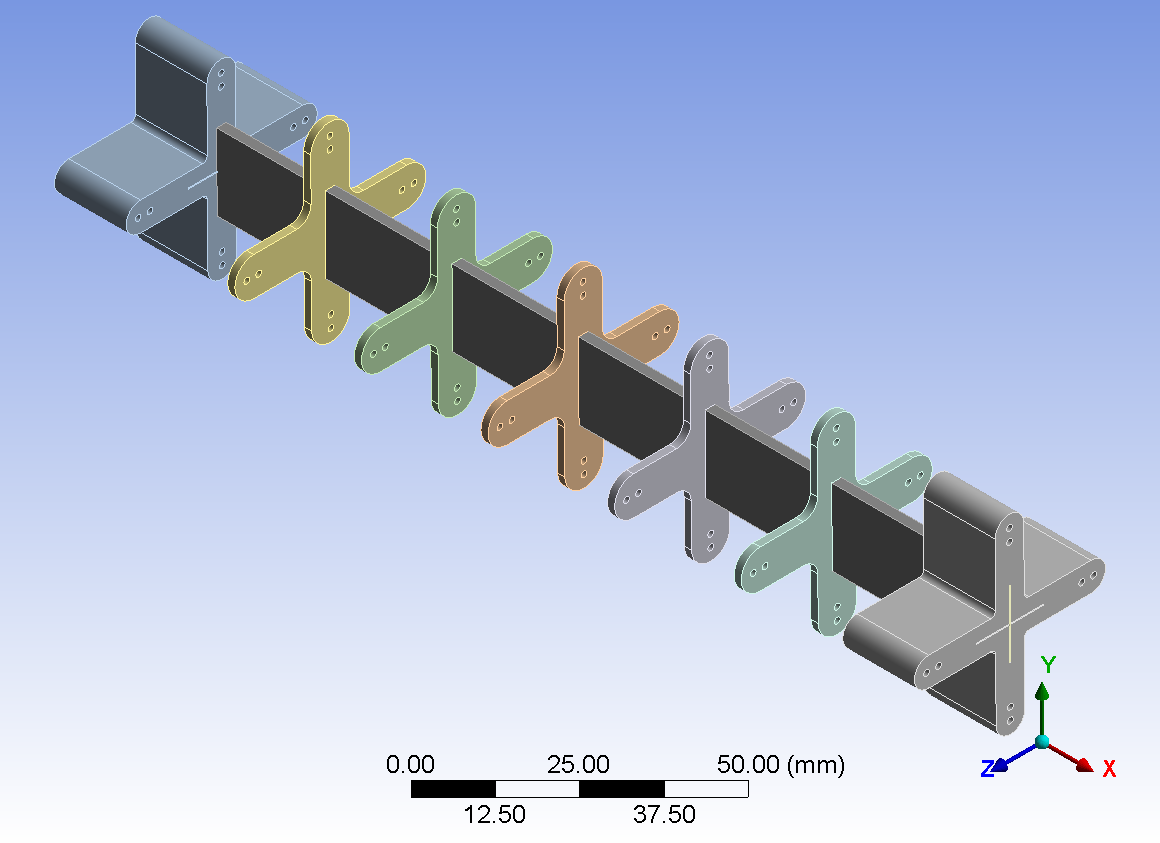
\includegraphics[width=.85\textwidth]{Image/Design/model.png} 
    \caption[The simplified model of manipulator]
    {\centering \textbf{The simplified model of manipulator.}}
    \label{fig:sim_model}
\end{figure}
\noindent Load it into ANSYS and use the Static Analysis Module to evaluate the stresses and strains at a maximum bending 
angle of 73 degrees.

To ensure that the results of the simulation are independent of the mesh size, a mesh-independent study is required. 
Finite element analyses were performed with mesh sizes ranging from 8.5 mm down to 2.5 mm. As illustrated in 
Figure \ref{fig:mesh_indep} a significant peak in stress at a mesh size of 6.5 mm suggests possible numerical artifacts or 
unresolved stress concentrations. Subsequent refinement below this threshold showed the stress values approaching 
a constant level, indicating the potential achievement of mesh independence.
\begin{figure}[H] % figure
    \centering
    \captionsetup{labelsep=colon}
    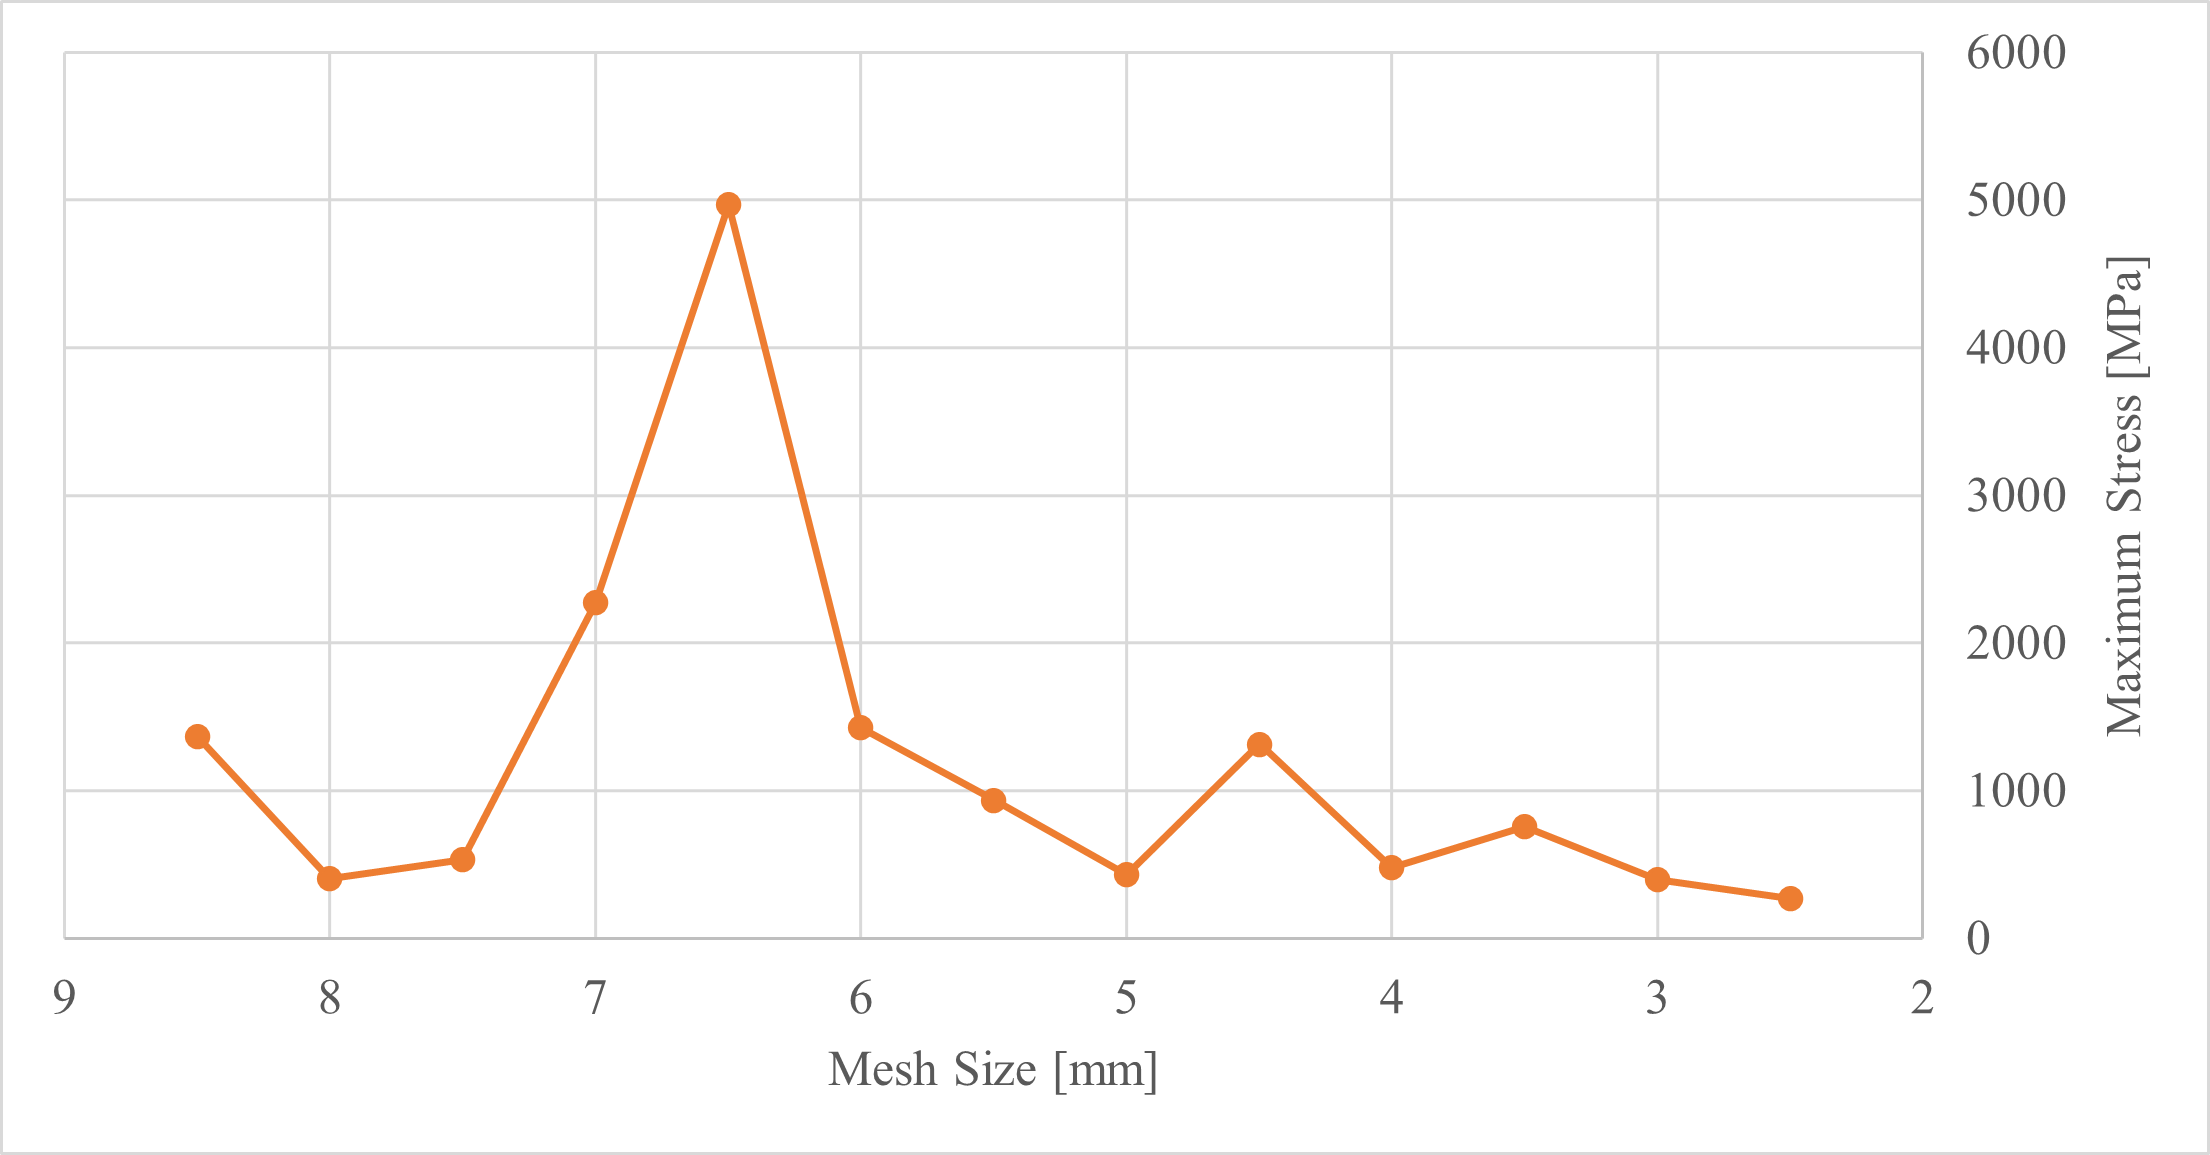
\includegraphics[width=.85\textwidth]{Image/Design/mesh_independence.png} 
    \caption[The mesh independence table]
    {\centering \textbf{The mesh independenc table.}}
    \label{fig:mesh_indep}
\end{figure}
\begin{figure}[H] % figure
    \centering
    \captionsetup{labelsep=colon}
    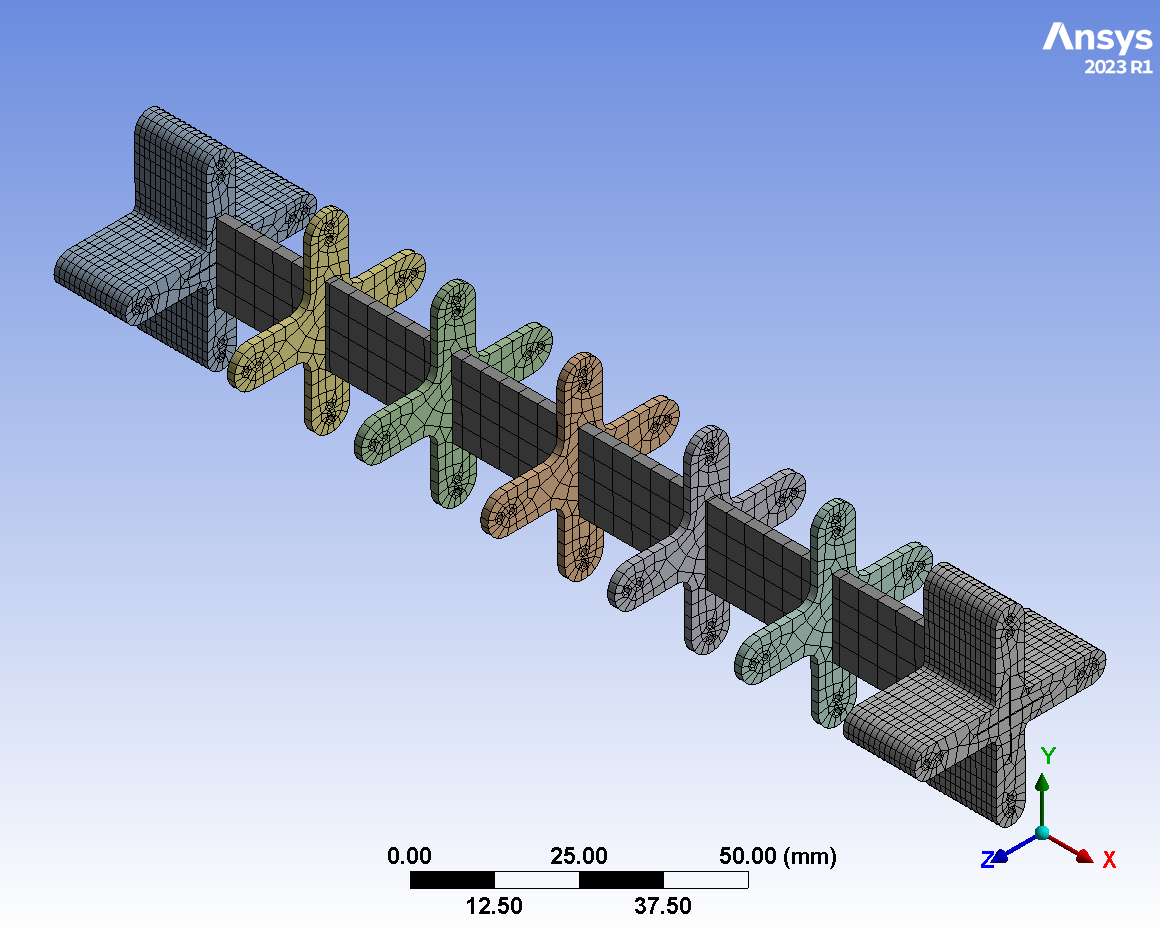
\includegraphics[width=.85\textwidth]{Image/Design/model_mesh.png} 
    \caption[The mesh model of manipulator]
    {\centering \textbf{The mesh model of manipulator.}}
    \label{fig:mesh_model}
\end{figure}
\noindent The trend toward constant stress values for mesh sizes finer than 4 mm suggests that the mesh is sufficiently 
detailed to capture the stress distribution within the component accurately. This finding establishes that a 
mesh size of 4 mm provides a balance between computational efficiency and the accuracy of the stress predictions. 
Based on these outcomes, a mesh size of 4 mm is used for further analysis, ensuring that the results are both 
computationally economical and reliable for engineering judgments. Figure \ref{fig:mesh_model} shows the mesh 
of the model.
%%%%% Forward Kinematics %%%%%
\subsubsection{Forward Kinematics}
The forward kinematics (FK) provided by Zhou et al. \cite{fishboneCR} were solely focused on a single segment 
with two modules. However, utilizing the FK algorithm for calculation became complex while there were four modules in 
the manipulator. The FK algorithm was rederived to generalize the workspace of the manipulator. 
\begin{figure}[H] % figure 
    \centering
    \captionsetup{labelsep=colon}
    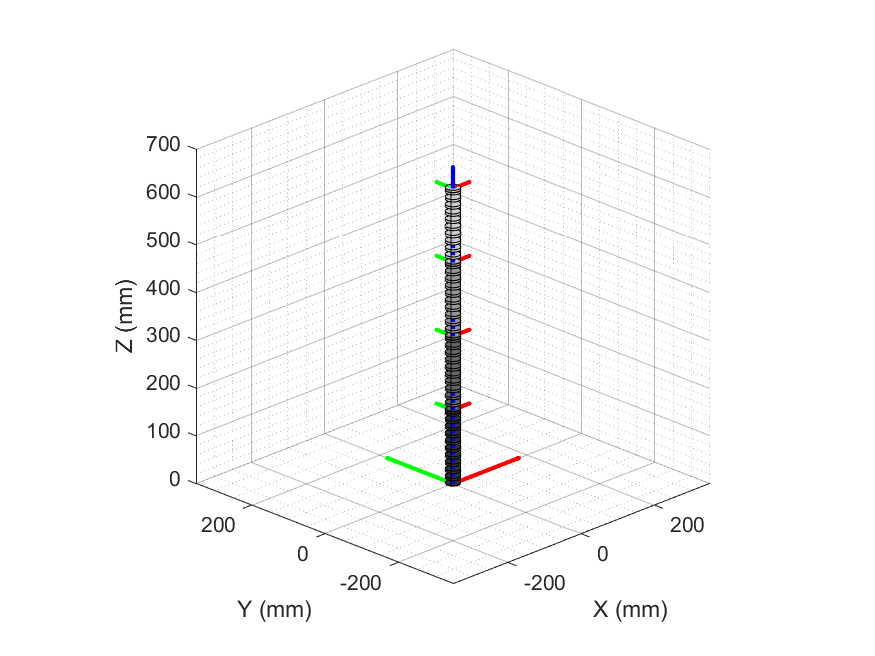
\includegraphics[width=1.0\textwidth]{Image/MATLAB/manipulator_0_0_0_0.png} 
    \caption[The kinematics model of manipulator at the initial position]
    {\centering \textbf{The kinematics model of manipulator at initial position.}}
    \label{fig:kinematics model 0_0_0_0}
\end{figure}
The base coordinate system (CS) was established with the centroid of base connector upper surface serving as 
the origin. The backbones of Module 1 and 3, which are Module (2,2) and (2,1), were parallel to the X-axis 
of base CS, while the backbones of Module 2 and 4, which are Modules (1,2) and (1,1), were parallel to the 
Y-axis of base CS. The upper surface centroids of connectors were designated as $node_1$, $node_2$, $node_3$, 
$node_4$, and $node_5$. The initial posture with CSs originated at $node_1 \sim node_5 $ are shown in 
Figure \ref{fig:kinematics model 0_0_0_0}. 

The Module 1 was restricted to bending in Y-Z plane of CS whose origin is $node_1$, while 
the Module 2 was restricted to bending in X-Z plane of CS whose origin is $node_2$. Similarly, the Module 
3 and 4 were subject to the same constraints. The right angle bending postures of single modules are 
illustrated in Figure \ref{fig:kinematics_model_resp}.
\begin{figure}[H] % figure
    \centering 
    \captionsetup{labelsep=colon}
    \begin{subfigure}{0.48\textwidth} % subfigure 1
        \centering
        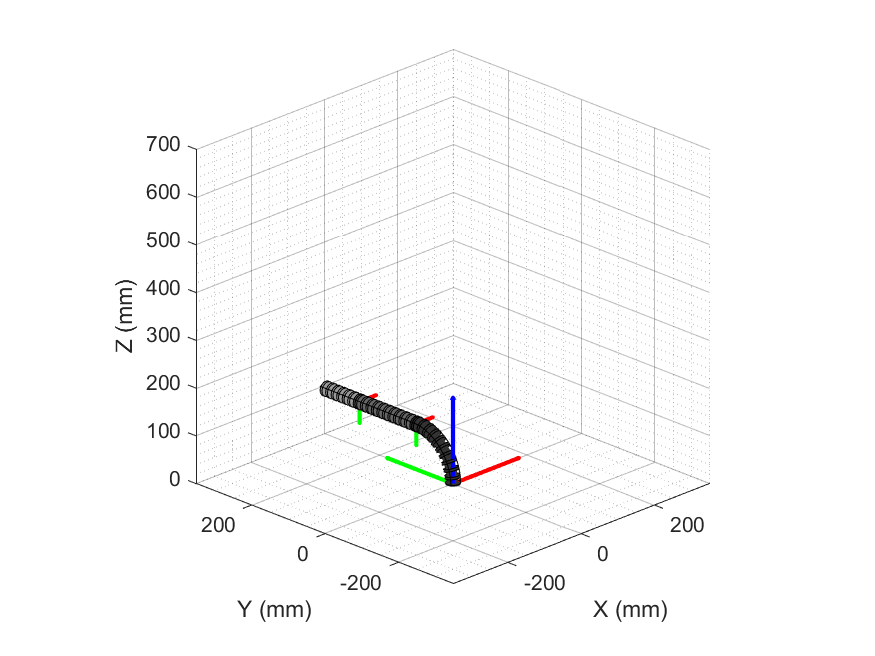
\includegraphics[width=\linewidth]{Image/MATLAB/manipulator_90_0_0_0.png}
        \caption{$\alpha_1=90 \degree,\alpha_2=0,\alpha_3=0,\alpha_4=0$}
    \end{subfigure}
    \hfill
    \begin{subfigure}{0.48\textwidth} % subfigure 2
        \centering
        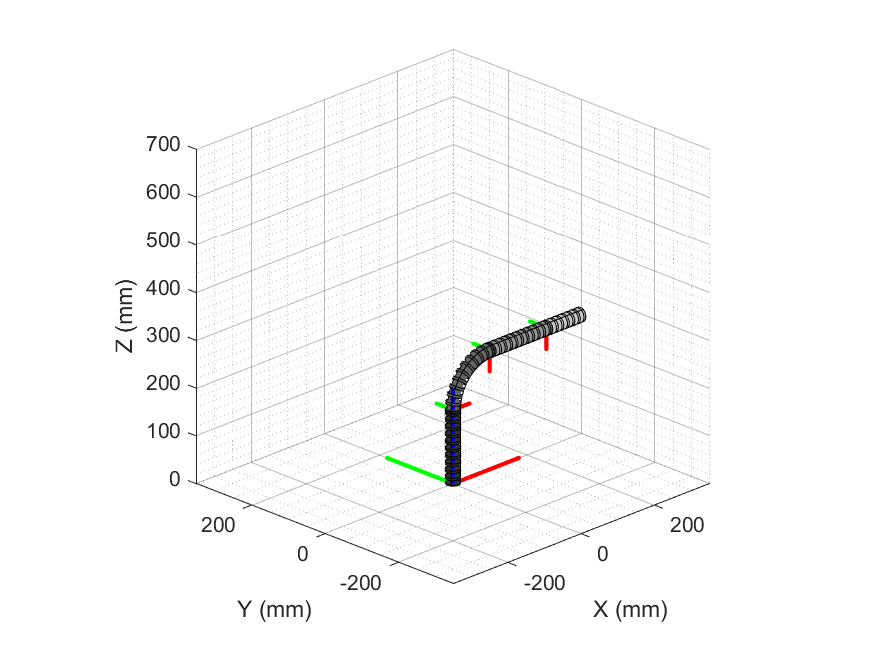
\includegraphics[width=\linewidth]{Image/MATLAB/manipulator_0_90_0_0.png}
        \caption{$\alpha_1=0,\alpha_2=90 \degree,\alpha_3=0,\alpha_4=0$}
    \end{subfigure}
    \begin{subfigure}{0.48\textwidth} % subfigure 3
        \centering
        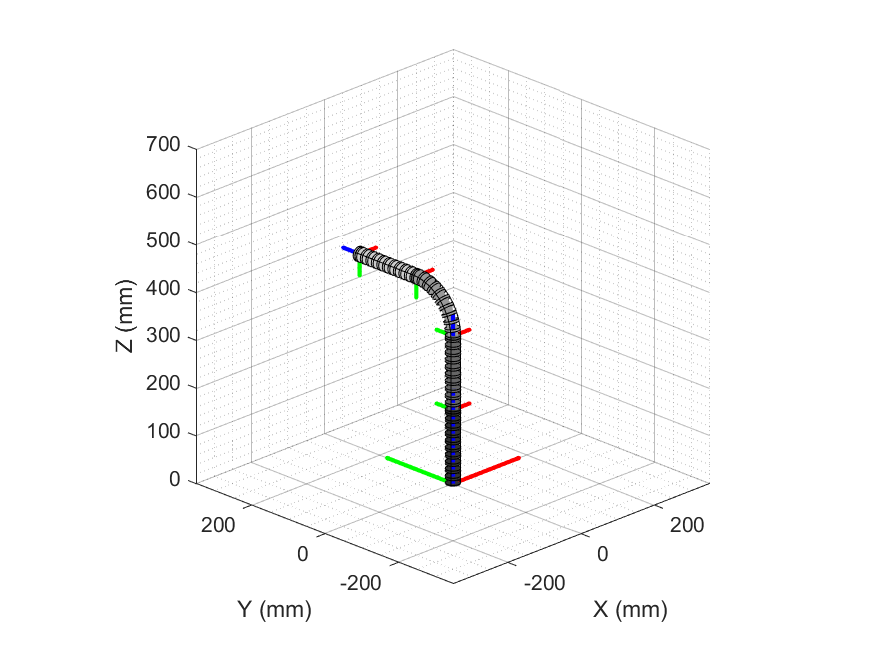
\includegraphics[width=\linewidth]{Image/MATLAB/manipulator_0_0_90_0.png}
        \caption{$\alpha_1=0,\alpha_2=0,\alpha_3=90 \degree,\alpha_4=0$}
    \end{subfigure}
    \hfill
    \begin{subfigure}{0.48\textwidth}
        \centering
        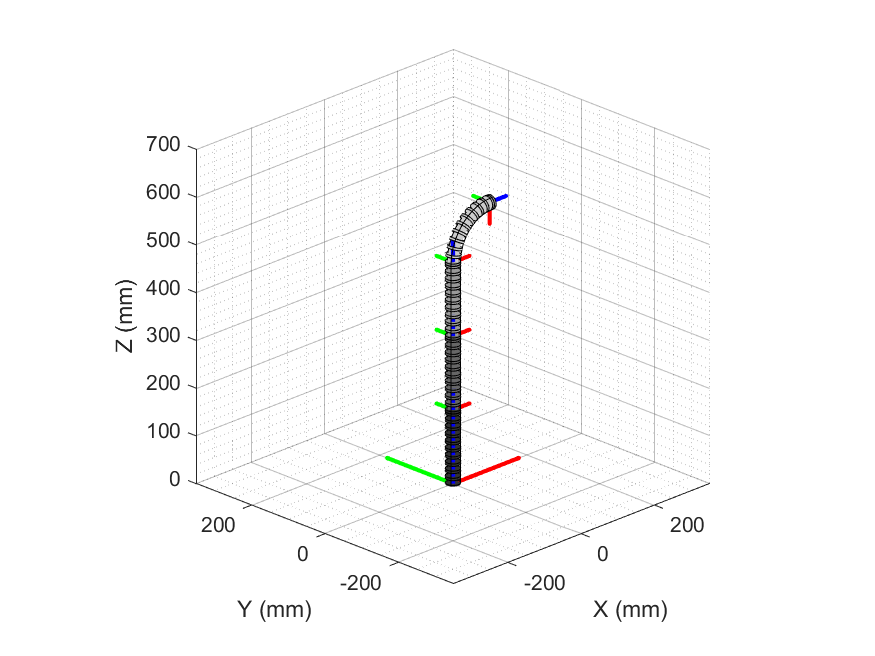
\includegraphics[width=\linewidth]{Image/MATLAB/manipulator_0_0_0_90.png}
        \caption{$\alpha_1=0,\alpha_2=0,\alpha_3=0,\alpha_4=90 \degree$}
    \end{subfigure}
    \caption[The right angle bending postures of single modules]
    {\centering \textbf{The right angle bending postures of single modules.}}
    \label{fig:kinematics_model_resp}
\end{figure}
The bending angle $\alpha$ was defined to be positive while the module bent toward positive 
direction of the X-axis or Y-axis. Owing to the distinct properties of the four modules, diverse calculation 
methods were utilized. The Module $i$ has a base node $node_i$ and an end effector node $node_{i+1}$. 
The position of $node_{i+1}$ in CS whose origin is $node_{i+1}$ was calculated in Equation 
\ref{eq:node i+1 calculation}. The detailed derivations are listed in Seciton \ref{sec:FK}.
\begin{align}
    &\textbf{P}_{i+1}^{base} = \textbf{R}_{i} \times \textbf{P}_{i+1}^{i} + \textbf{P}_{i}^{base}
    \label{eq:node i+1 calculation}
\end{align}
\vspace{-18mm}
\begin{align*}
    &\ \textbf{P}_{i+1}^{base}\text{: The absolute position matrix (APM) of $node_{i+1}$ in the base CS.}\\
    &\ \textbf{R}_{i}\text{: The rotational matrix transforms the base CS into CS \textit{i} whose origin is $node_i$.}\\
    &\ \textbf{P}_{i+1}^{i}\text{: The relative position matrix (RPM) of $node_{i+1}$ in CS \textit{i}.}\\
    &\ \textbf{P}_{i}^{base}\text{: The absolute position matrix (APM) of $node_{i}$ in the base CS.}
\end{align*}

Applying the corresponding transformations to the Equation \ref{eq:node i+1 calculation} revealed the patterns shown 
in Equations \ref{eq:nodei+1_position_absolute_minus} and \ref{eq:nodei+1_position_absolute}.
\vspace{-5mm}
\begin{align}
    &\textbf{P}_{i+1}^{base} - \textbf{P}_{i}^{base} = \prod_{n=1}^{i}\textbf{R}_{n}\times \textbf{P}_{i+1}^{i} 
    \label{eq:nodei+1_position_absolute_minus} \\
    &\textbf{P}_{i+1}^{base} = \sum_{m=1}^{i}\left[\prod_{n=1}^{m}\textbf{R}_{n}\times \textbf{P}_{m+1}^{m}\right] \quad(\textbf{P}_{1}^{base} = 0)
    \label{eq:nodei+1_position_absolute}
\end{align}
\vspace{-5mm}
%%%%% Inverse Kinematics %%%%%
\subsubsection{Inverse Kinematics}
The inverse kinematics (IK) algorithm was inspired by a rigid manipulator IK solver called FABRIK 
\cite{fabrik}. W. Zhang et al.\cite{fabrikc} expanded this solver to the continuum manipulator domain. Considering 
the distinctive nature of the manipulator, adaptations were implemented to the FABRIKc solver, transforming it 
into a tailored IK algorithm for this particular application. For further elucidation, the IK derivation was 
demonstrated using a target whose angles $\boldsymbol{target}$ = [0,0,90,0] $\degree$. The comprehensive process 
of the first epoch will be elaborated as follows. Simultaneously, the flowchart of IK algorithm was shown in 
Figure \ref{fig:flowchart}. 

\begin{figure}[H]
    \centering
    \captionsetup{labelsep=colon}
    \begin{tikzpicture}[node distance=1.5cm,every node/.style={fill=white, font=\sffamily}, align=center]
        % Specification of nodes (position, etc.)
        \node (input) [data]   
        {\textbf{Input}: $\textbf{O}_{target}$, $\textbf{P}_{target}$, $\boldsymbol{\epsilon}$, ${\textbf{Epoch}}_{max}$ };
        \node (start) [activityStarts, below of=input, yshift=1mm] {Start};
        \node (init) [process, below of=start, yshift=1mm]          
        {Initialization: $\textbf{vnode}_i$, $\textbf{node}_i$, $\textbf{l}_i$};
        \node (value) [process, below of=init, yshift=1mm]   
        {\textbf{Epoch} = 1, $\textbf{e} = \lVert\textbf{P}_{target} - \textbf{P}_{\boldsymbol{\theta}}\rVert$};
        \node (deter) [pending, below of=value, yshift=-20mm]   
        {$\textbf{e} > \boldsymbol{\epsilon}$ \text{AND} \\ $\textbf{Epoch} < {\textbf{Epoch}}_{max}$};
        \node (frp) [process, below of=deter, yshift=-25mm, fill=red!25] {FABRIKc: Forward Reaching Phase};
        \node (brp) [process, below of=frp, fill=red!25] {FABRIKc: Back Reaching Phase};
        \node (plus) [process, below of=brp] {\textbf{Epoch} = \textbf{Epoch} + 1};  
        \node (deter_epo) [pending, right of=deter, xshift=55mm] {$\textbf{Epoch} > {\textbf{Epoch}}_{max}$};  
        \node (fail) [data, above of=deter_epo, yshift=25mm] {\textbf{Output}: $\boldsymbol{\theta}$ with min $\textbf{e}$};  
        \node (success) [data, below of=deter_epo, yshift=-25mm] {\textbf{Output}: $\boldsymbol{\theta}$ with $\textbf{e}$ and $\textbf{Epoch}$}; 
        \node (deltaS) [data, below of=success, yshift=-10mm] {\textbf{Output}: $\boldsymbol{\Delta S}$};  
        % Specification of lines between nodes specified above
        % with aditional nodes for description 
        \draw[->]  (input) -- (start);
        \draw[->]  (start) -- (init);
        \draw[->]  (init) -- (value);
        \draw[->]  (value) -- (deter);
        \draw[->]  (deter) -- node {Yes}(frp);
        \draw[->]  (frp) -- (brp);
        \draw[->]  (brp) -- (plus);
        \draw[->]  (plus) -- ++(-3.6,0) -- ++(0,7.0) -- (deter);
        \draw[->]  (deter) -- node {No}(deter_epo);
        \draw[->]  (deter_epo) -- node {Yes}(fail);
        \draw[->]  (deter_epo) -- node {No}(success);
        \draw[->]  (success) -- node {conversion}(deltaS);
        \draw[->]  (fail) -- ++(3.0,0) -- node {conversion} ++(0,-10.5) -- (deltaS);
    \end{tikzpicture}
    \caption[The flow chart of the IK algorithm]
    {\centering \textbf{The flow chart of the IK algorithm.}}
    \label{fig:flowchart}
\end{figure}
The orientation and position matrices of the target were derived in Equation 
\ref{eq:target_homo}. These matrices were utilized as the input of the IK algorithm. The output of the algorithm 
was a series of bending angles $\boldsymbol{\theta}$.
\vspace{-5mm}
\begin{align}
    \textbf{O}_{target} = 
    \begin{bmatrix}
        1 & 0 & 0 \\
        0 & 0 & -1 \\
        0 & 1 & 0 \\
    \end{bmatrix} 
    \qquad
    \textbf{P}_{target} = 
    \begin{bmatrix}
        0 \\
        245.493 \\
        395.493 \\
    \end{bmatrix} 
    \label{eq:target_homo} 
\end{align}

Additionally, it is essential to introduce a novel concept called "virtual node". This raised the fact that FABRIK 
algorithm was originally designed for rigid manipulators, which implied that continuum manipulators need to be abstracted 
for modeling purpose. In this context, the module of manipulator were abstracted as a rigid manipulator with two prismatic 
joints and one revolute joint. The location of the revolute joint served as the virtual node. 

Subsequently, the forward reaching phase of the FABRIKc algorithm can commence. The calculation which involves four 
iterations was specified in Section \ref{sec:IK}.

Ultimately, the FABRIKc algorithm initiated the backward reaching phase, which is the FK algorithm. The 
FABRIKc algorithm inherently guaranteed the orientation of manipulator's end effector,  with the necessity to account 
solely for positional errors. The error was calculated by Equation \ref{eq:error_calculation}.
\vspace{-5mm}
\begin{align}
    \textbf{e} = \lVert\textbf{P}_{target} - \textbf{P}_{\boldsymbol{theta}}\rVert
    \label{eq:error_calculation}
\end{align}
For the first epoch, the results of IK algorithm were
$\boldsymbol{\theta} = [6.71,\ -0.0,\ 83.29,\ -0.0]\degree $, 
The error of the first epoch was 33.77506. The results about IK algorithm with the target angle 
$\boldsymbol{\alpha} = [0,\ 0,\ 90,\ 0] $ are shown in Table \ref{tab:fabrikc_0_0_90_0} 
in Appendix \ref{append:table}. The algorithm was configured to execute a maximum of 200 epochs, with 
the provision to pause when the error reaches a sufficiently low level, thereby conserving computational resources. 
The maximum epoch number was defined as ${\textbf{Epoch}}_{max}$.
%%%%% Angular Conversion %%%%%
\subsubsection{Angular Conversion}
The Arduino programme utilized $\boldsymbol{\Delta S}$ as input to control the motors. However, the solutions of IK 
algorithm are $\boldsymbol{\theta}$, which are angles. It is vital to convert angles $\boldsymbol{\theta}$ 
into $\boldsymbol{\Delta S}$. The variables $R_1$, $R_2$, and $R_3$ were mentioned in Equations 
\ref{eq:node2_postion_relative}, \ref{eq:node3_postion_relative}, and \ref{eq:node4_postion_relative}, while 
$R_4 = {Sr}_4/ \alpha_4$. The relationship between $\boldsymbol{\theta}$ and $\boldsymbol{\Delta S}$ was shown in 
Equation \ref{eq:deltaS}. The relationship can be further generalized into matrix in Equation \ref{eq:deltaS_matrix} 
for Python programme.
\vspace{-5mm}

%%%%% ELECTRONIC CONTROL %%%%%
\subsection{Electronic Control}
%%%%% Actuation Control %%%%%
\subsubsection{Actuation Control}
As mentioned above, the manipulator is divided into four units in total, with each unit being controlled for its 
bending movements by two cables. This means that the entire manipulator is controlled by a total of 8 cables. How 
to control the extension and retraction of these 8 cable ropes is the key to the Control part. 

In this project, 8 stepper motors are employed to control the 8 individual cables. The planned design involves 
wrapping the cables around the rotor of each motor, and the stepper motors are programmed to extend or retract 
the ropes by stepping a certain number of steps in either a counterclockwise or clockwise direction. These 8 motors 
are connected to an Arduino board together, and the user can control the programme by a keyboard, and a serial monitor. 
\begin{itemize}
    \item Actuation Principle\\
    In this programme, the user inputs the desired length changes for 8 cables $\Delta S_1$ ~ $\Delta S_8$ 
    ($\Delta S_{1,2,3,4}$ ranging from -36.65 mm to 36.65 mm, $\Delta S_{5,6,7,8}$ ranging from -68.07 to 68.07 mm). 
    After conversion, it outputs the corresponding step numbers $Step_1$ ~ $Step_8$ for the eight stepper motors. 
    Based on this, the 8-stepper motors will step correspondingly. The relationship between the changes in 
    cable length and the motor steps can be defined by Equation \ref{eq:step_motor_arduino}. 
    
    \vspace{-5mm}
    \begin{align}
        & \qquad\qquad\qquad\qquad Step_i=\frac{(\Delta S_i-\Delta S_{i(prev)})\cdot N}{\pi\cdot d}, \ i\in[1,8] 
        \label{eq:step_motor_arduino} \\
        &\Delta S_{i(prev)} \text{: The length change for $i^{th}$ cable in the previous location.} \nonumber \\
        &d\text{: The diameter of the rotor. A rotor of diameter 10 mm is used currently.} \nonumber \\
        &N\text{: Number of steps/rev. 2048 for 28YBG-48 motor.}\nonumber 
    \end{align}
    \vspace{-15mm}
    \item Component Selection \\
    To achieve a successful and precise control functionality, the first thing to do is to select appropriate 
    components. The list below shows the main electronic components used:
    \begin{itemize}
        \item Arduino Mega 2560 board: \\
        The Arduino Mega 2560 is the most suitable board since it boasts up to 54 I/O pins and a more powerful 
        processor to allow for better performance in multitasking operations \cite{arduino_guide}.
        \item 28YBJ-48 stepper motor: \\
        The 28YBJ-48 stepper motor is currently one of the most commonly used stepper motors on the market. It is capable to rotate
         in rather 4096 steps/rev or 2048 steps/rev. This high-resolution configuration allows the 
        manipulator to perform high-precision operations. Additionally, at its rated voltage, it can provide 
        a torque of up to 34Nm, which is more than sufficient for pulling the cables of a lightweight manipulator.
        \item ULN 2003A motor control chip: \\
        The motor control chip acts as the brain of the motor, responsible for translating instructions from the 
        Arduino board into operations that the motor can execute. The ULN2003A chip is specifically matched with 
        the 28YBJ-48 motor, ensuring seamless coordination and operation between the chip and the motor. 
        \item 9V power supply: \\
        The rated operating voltage of the stepper motor is 5-12V. Here, a 9V power supply is chosen to allow 
        losses due to component resistance. 
    \end{itemize}
    \item Circuit Schematics \\
    The schematic of the overall circuit for the manipulator actuation control part is shown in 
    Figure \ref{fig:motor_circuit_layout} in Appendix \ref{append:figures}. \\
    The 8 motors use pin 22-52 on the Arduino Mega 2560 board, and are powered by a 9V battery in parallel order. The Arduino 
    board is connected to a serial monitor and a keyboard for state inspection and manual input.
    \item Programme development \\
    The main logic framework of the programme has been illustrated by the flowchart shown in Figure \ref{fig:motor_flowchart}. 
    \vspace{-5mm}
    \begin{figure}[H] % figure
        \centering 
        \captionsetup{labelsep=colon}
        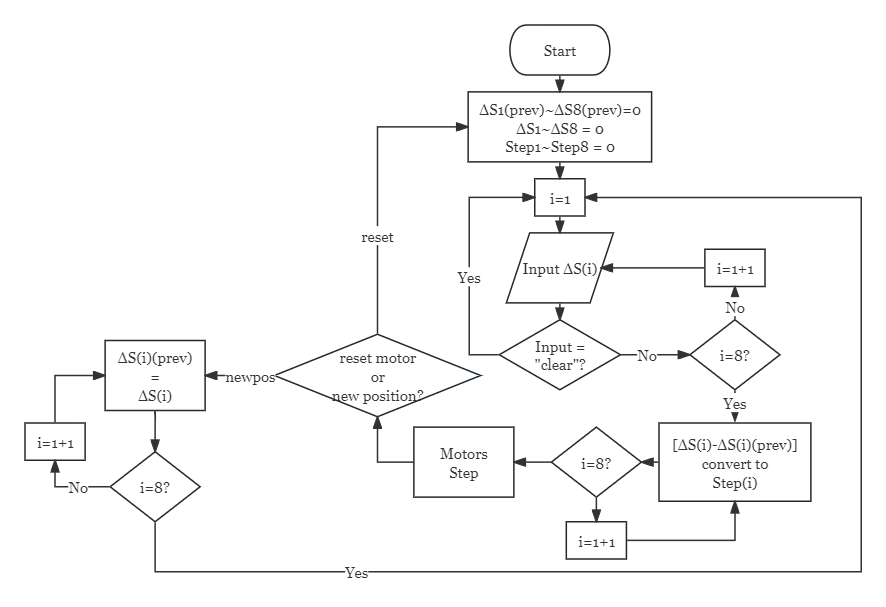
\includegraphics[width=1.0\textwidth]{Image/Design/flowchart_arduino_motor.png} 
        \caption[The flow chart of Arduino step motor control programme]
        {\centering \textbf{The flow chart of Arduino step motor control programme.}}
        \label{fig:motor_flowchart}
    \end{figure}
    After the programme starts, the first thing is to declare the variables. $\Delta S_{i(prev)}$, $\Delta S_i$ and 
    $Step_i$ is all set to 0 initially. Then the programme asks the users to input 8 numbers representing the 
    length change for 8 cables which will be assigned to variable $\Delta S_1$ ~ $\Delta S_8$ in order. 
    During the input process, the user can input `clear' instead of numbers to clear all the previous input and 
    start over again from $\Delta S_1$. \\
    Once the input process is complete, the programme converts the $\Delta S_1$~$\Delta S_8$ to $Step_1$ ~ $Step_8$ 
    based on Equation \ref{eq:step_motor_arduino}, with the $d$ set to 10 mm, N set to 2048 steps/rev. The motors 
    will start to step immediately after the conversion is finished. \\
    During the stepping process, the motors controlling the first and second unit (the first 4 motors) are set 
    to have a stepping speed of 300 steps/second, and the motors controlling the third and fourth unit 
    (the last 4 motors) are set to have $\frac{300}{17.5}\cdot(17.5+15)\approx 557$ steps/second. This is because 
    the moving speed for the last two units should be $\frac{17.5+15}{17.5}$ times faster than the first two units 
    so that the 4 units can finish moving approximately at the same time. \\
    The programme shall wait until the motors finished stepping. Once the stepping process is finished, the programme 
    asks the user what to do next: reset the motors to initial position or move from the current position to the 
    next position. If the user chooses to reset the motors, all the motors rotate backwards for same steps. 
    However, If the user chooses to let the motors move to a new position, the values for current $\Delta S_1$ ~ 
    $\Delta S_8$ will be stored to variable $\Delta S_{1(prev)}$ ~ $\Delta S_{8(prev)}$. The programme then asks for 
    a new set of $\Delta S_1$ ~ $\Delta S_8$, then calculate the new $Step_1$ ~$Step_8$. Hence, the logic loop of the 
    programme is closed.
\end{itemize}
%%%%% Parameter Input %%%%%
\subsubsection{Parameter Input by Serial Monitor}
In the operating logic, the control parameters are inputted through the keyboard to control the motion of the 
multiple stepper motors. The basic function is to input the steps into the serial monitor through the keyboard 
of the host computer and the input string will be read by the microcontroller and converted into data, which are 
used as the number of steps of the stepper motor movement. For easy operation and display, the input parameters 
need to be displayed as text on the serial monitor, as well as on the screen of the LCD IIC (when serial monitor is not available). 
LCD IIC will be in the form of a 2-line, 16-bit display to show more content. 

The logic flowchart of the code to control the motor and LCD IIC by inputting parameters with the serial monitor of 
the host computer is shown in Figure \ref{fig:cl_input} in Appendix \ref{append:figures}.
%%%%% MPU 6050 %%%%%
\subsubsection{Verification of MPU 6050}
According to the project content, adding sensors to the end effector to measure its orientation angle and distance 
from the contact plane can assist the user to carry out more accurate operation. The function of detecting the 
orientation angle is realised by the MPU6050.

The Orientation angle (Euler angle) corresponding to the MPU6050 chip is shown in Figure \ref{fig:mpu6050_chip}. 
Pitch is rotation around the X-axis. Yaw is rotation around the Y-axis. Roll is rotation around the Z-axis. 
\begin{figure}[H] % figure
    \centering
    \captionsetup{labelsep=colon}
    \begin{subfigure}{0.45\textwidth} % subfigure 1
        \centering
        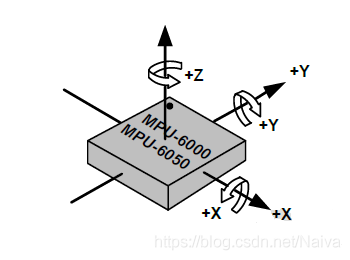
\includegraphics[width=\linewidth]{Image/Design/MPU6050_chip.png}
        \caption{\centering The MPU6050 chip corresponding to the Euler angle}
        \label{fig:mpu6050_chip}
    \end{subfigure}
    % \hfill
    \begin{subfigure}{0.45\textwidth} % subfigure 2
        \centering
        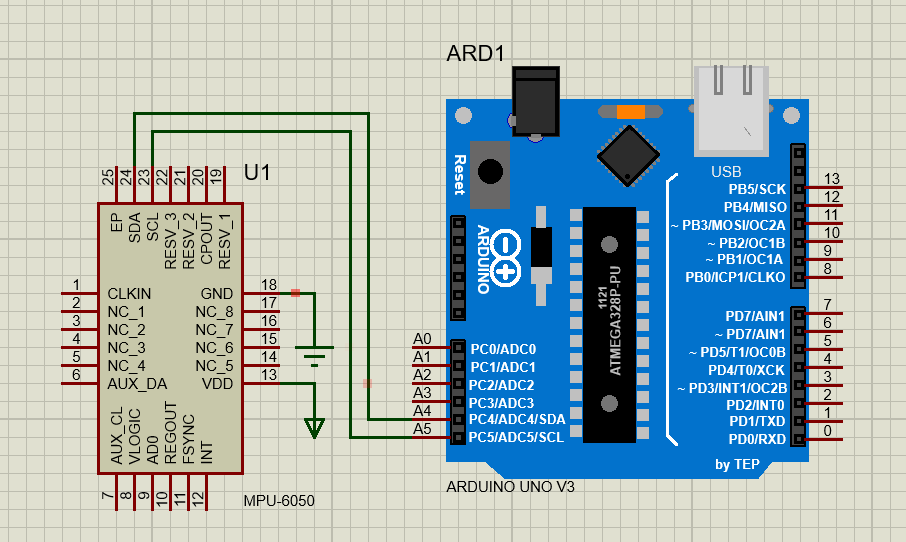
\includegraphics[width=\linewidth]{Image/Design/MPU6050_circuit.png}
        \caption{\centering The wiring diagram of MPU6050 and microcontroller}
        \label{fig:mpu6050_circuit}
    \end{subfigure}
    \caption[The MPU6050 chip with ancillary Arduino circuit]
    {\centering \textbf{The MPU6050 chip with ancillary Arduino circuit.}}
    \label{fig:mpu6050}
\end{figure}
\vspace{-5mm}

The MPU6050 requires an external 5V power supply and GND. SCL is the Clock Pin of the IIC when the 
MPU6050 is used as a slave, and SDA is the Data Pin of the IIC when the MPU6050 is used as a slave. The wiring 
diagram is shown in Figure \ref{fig:mpu6050_circuit}. 

The logic flowchart of the code that controls the MPU 6050 to display acceleration and direction angle is shown 
in Figure \ref{fig:cl_angle} in Appendix \ref{append:figures}. In this project, the acceleration parameters will 
not be acquired and displayed.

Since Proteus does not support dynamic simulation of the MPU6050, the verification of the MPU6050 has been 
carried out by physical components and Arduino Mega while the project is in progress.  
%%%%% HC-SR04 %%%%%%
\subsubsection{Using HC-SR04 to measure distance}
The HC-SR04 Ultrasonic Sensor uses sonar to determine the distance to an object. It has an ultrasonic 
transmitter and a receiver module which provides excellent non-contact range detection, high accuracy and 
stable readings. The measurement range is from 2 to 400 cm. The resolution is 0.3 cm and the measurement angle 
is within 30°.

The sensor is triggered by sending a HIGH pulse of 10 microseconds. Previously, the speaker gives a short 
low-level pulse to ensure a clean HIGH pulse is obtained. 
The basic principle of distance measurement is Time-of-Flight (ToF). The formula is as follows.
\vspace{-10mm}
\begin{align}
    distance = (duration/2) \times v_{sound} \\
    \text{(}v_{sound} = 343\ m/s = 1/29.1\ cm/us \text{)}\nonumber
\end{align}
The wiring diagram and simulation results are shown in Figure \ref{fig:tof}. An SSD 1306 OLED screen 
is used to display the data in the simulation. The logic flowchart of the code that controls the HC-SR04 to measure 
distance and display acceleration by OLED screen is shown in Figure \ref{fig:cl_tof} in Appendix \ref{append:figures}.
\begin{figure}[H] % figure
    \centering 
    \captionsetup{labelsep=colon}
    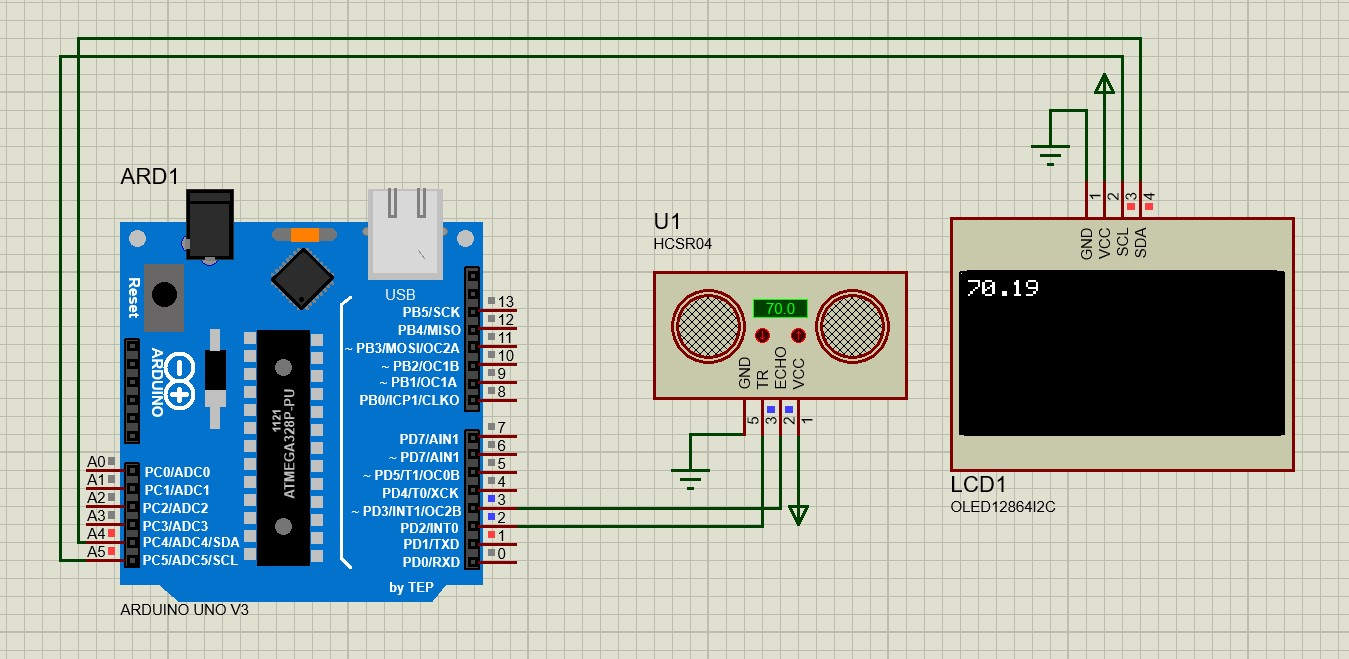
\includegraphics[width=0.9\linewidth]{Image/Design/tof_circuit.jpg}
    \caption[The wiring diagram and simulation of HC-SR04]
    {\centering \textbf{The wiring diagram and simulation of HC-SR04.}}
    \label{fig:tof}
\end{figure}

%%%%% OLED Screen %%%%%
\subsubsection{SSD 1306 OLED}
Using SSD 1306 OLED requires calling two libraries, \lstinline{<Adafruit_SSD1306.h>} and 
\lstinline{<Adafruit_GFX.h>}. \lstinline{<Adafruit_SSD1306.h>} is a dedicated display library for SSD1306 OLED 
screens. \lstinline{<Adafruit_GFX.h>} library is the common parent graphics library for LCD and OLED screens. 

The resolution of SSD1306 is 128x64 pixel dot array, with clock, data, power pins required. Figure \ref{fig:cl_oled} in 
Appendix \ref{append:figures} is the logic flowchart of the code to control the OLED to display the text content. 
\newpage

% change to new page
\newpage 